\chapter{Basic Postulates of Relativity}
\label{chapter:relativityI}

%\section*{Objectives}
%\begin{objectives}
%\item Be able to state the basic, fundamental principles of
%  relativity, and be able to explain how the various aspects of
%  relativity all follow logically from these basic principles.
%
%\item Know how and when to use the proper time relation to relate time
%  intervals in two different reference frames.
%
%\item Be able to relate length and distance measurements in two
%  different reference frames using length contraction.
%
%\item Be able to transform velocities from one reference frame to
%  another.
%\end{objectives}

\section{Introduction}

Certain numbers immediately bring to mind thoughts or ideas.  For
example, ``101'' makes people think of spotted puppies, ``747''
engenders thoughts of large airplanes, ``911'' is the number that you
call for an emergency or one of the worst dates in the history of our
country, and ``42'' is the answer to the ultimate question of Life,
the Universe and Everything.  And if you mention the number ``1905''
to any physicist, he/she will immediately think of the year in which
Albert Einstein published three papers that completely revolutionized
science and fundamentally changed the way in which we view the
universe.  The first paper\footnote{A. Einstein, Annalen der Physik
  {\bf 17}, 132 (1905).} introduced the idea of photons (particles of
light), an idea which formed one of the cornerstones of quantum
mechanics.\footnote{Interestingly, even though any one of these papers
  would be a monumental lifetime achievement for any mere mortal
  physicist, Einstein received the Nobel prize in physics only for his
  work on photons.}  (You will learn about this next semester in PHYS
212.)  The second paper\footnote{A. Einstein, Annalen der Physik {\bf
    17}, 549 (1905).}  was the first to connect molecular diffusion
--- spreading of an impurity in a motionless fluid --- with random
Brownian motion of the individual impurity molecules, which is regarded
as the first demonstration of the existence of atoms.
   
The third paper had a innocuous title: ``On the electrodynamics of
moving bodies.''\footnote{A. Einstein, Annalen der Physik {\bf 17},
  891 (1905).} But there is nothing even remotely innocuous about the
implications of the theory, now known as Einstein's Special Theory of
Relativity (``special relativity'' for short), presented in that
paper.  Einstein's theory completely changed our conceptions of time
and distance\footnote{\dots and, in fact, establishes that they are
  profoundly related, as we shall see.} and of energy and
matter.\footnote{\dots and, in fact, establishes that they are
  profoundly related, as we shall see.}  The theory also led to an
explanation of how stars generate light --- the fundamental source of
energy in the universe without which life on this planet would not be
possible --- and led to the Earth-shattering (almost literally,
unfortunately) development of nuclear weapons.  The theory also holds
the key to the future development of non-fossil fuel energy sources.
Simply put, you cannot understand how the universe works without
studying Einstein's theory of relativity.
   
This chapter and the following three introduce the main ideas and
implications of the Special Theory of Relativity, which applies to the
motion of objects in {\em inertial} (non-accelerating, or ``free
float''\footnote{Taylor and Wheeler, {\it Spacetime Physics}, 2$^{\rm
    nd}$ Edition, (Freeman, 1992), p.\ 26.})  reference frames.  At the
end of the semester, we will also briefly discuss Einstein's General
Theory of Relativity (``general relativity'' for short), which expands
the theory to account for the effects of acceleration and
gravitational fields.

\section{Preliminaries}
A few definitions will be useful for the next few chapters.
   
An {\em event} is something that happens at a particular
location at a particular time.  It is important to be clear about
this, because relativity deals with how different observers measure
distances and times between events.  For instance, let's say that the
penguin on top of your television set explodes at 7:12 a.m.\ on a
Saturday morning.  You then run 5 km to a large tower where you
capture (at 7:45 a.m.) a small platypus that inexplicably is dressed like a
secret agent and who is trying to thwart your plans to take over
the Tri-State Area.  You could identify two events --- (1) the
explosion of the penguin and (2) your capture of the semi-aquatic,
egg-laying mammal of action (i.e., the platypus) --- and say
that these events are separated by 5 km in space and 33 min in time.
Relativity addresses the question of how a different observer measures
the distance and time between the same two events.  (Preview: not
everyone will agree about the distance and time between events.)
   
% And speaking of observers, we need to define a {\em reference
% frame}.  A reference frame can be thought of as a set of common
% observers subject to the same conditions.  Specifically, we will say
% that several observers are in the same reference frame if they agree
% about the distance and time between any two events.
   
So what do we mean, exactly, by ``different observers,'' and what
are the characteristics of these observers that will determine how
their measurements will differ?  We start by explaining what is meant
by the term ``reference frame.'' You can visualize a reference frame
as a set of rulers (distance measuring devices) and clocks (time
measuring devices) that are arrayed throughout space so that the
position and time of any event can be determined directly.  The distinguishing
feature of a reference frame is that the set of ``rulers'' and ``clocks''
are all at rest with respect to one another.  An observer IN THIS
REFERENCE FRAME is at rest with respect to all the rulers and clocks.
Notice that there can be many observers at different positions
in this reference frame, as long as they are all at rest with respect
to each other and to the measuring tools. All observers in the same
reference frame will agree with each other about the distances and
times between any two events, but they will not agree with observers
in other reference frames moving with respect to their frame.

A particularly important kind of reference frame is an {\em
inertial reference frame}.  Observers in an inertial reference
frame experience no significant acceleration, nor can they discern any
gravitational effects.  In an ideal inertial reference frame, the
observer would be floating free (hence the name ``free float'' that is
sometimes used to discuss an inertial reference frame), because any
non-floating motion would necessarily imply either acceleration or
gravitational effects.  To analyze behavior in the vicinity of very
strong gravitational fields, it is necessary to use general
relativity.
   
Technically, an observer is not in a true inertial reference frame if
she is standing on the surface of a planet since there is gravitation.
However, there are plenty of situations where non-inertial effects are
small enough as to be negligible.  In fact, the gravitation from a
typical planet is small enough so that the non-inertial effects are
negligible, and Special Relativity works perfectly well.  So, for
example, we will often treat observers moving on a constant velocity
train as though they are in an inertial reference frame, even though
there is a small gravitational effect.
   
When dealing with velocities, we have to be careful.  A velocity
technically has meaning only if there is a reference.  So, for
example, if you are in a car and you are traveling 65 mph toward the
West, you are really traveling 65 mph {\em relative to the
surface of the Earth}.  In fact, almost any velocity that people
quote in everyday usage is defined relative to the Earth.
   
\begin{boxittext}
{{\bf In preparation for class}, consider the following question: how
fast are you {\em really} going if you are in the car in the previous
paragraph?}
\end{boxittext}
   
Certainly, anyone who is willing to accept a non-geocentric view of
the universe realizes that there is nothing inherently special about
the earth as a reference frame.  But scientists have long wondered if
there is some preferred universal reference frame from which all
velocities should be defined, some standard by which we could define
{\em absolute velocities} for every object in the universe.
   
In relativity, we will use {\em relative velocities}, i.e.,
velocities will always be defined relative to some reference frame.
In fact, one result of relativity is the realization that this is the
best way to define velocity.  There is no need to choose any special
reference frame for the universe; all the results of relativity work
perfectly well with velocities measured relative to any reference
frame that you might choose.
   
The following statement applies to relative velocities: if observer A
measures observer B to be moving at a (relative) velocity of $\vec{v}$
in a particular direction, then B measures A to be moving at a
(relative) velocity of $-\vec{v}$; i.e., same speed but opposite
direction.

\section{Fundamental Principles of Relativity}

Einstein's Special Theory of Relativity is based on a very simple
premise, namely


\begin{boxittext} {{\bf The Principle of Relativity}: the laws of
    physics are the same for observers in different inertial reference
    frames.}
\end{boxittext}

\noindent Let's say, for example, that Michelle sets up a lab in the
basement of Olin Science while Barack sets up an identical lab inside
a truck that is driving on Route 15 with a constant velocity.
Whatever physics equations (including fundamental constants) Michelle
uses to predict and describe the behavior in her lab should work
equally well for Barack in his lab.

Not only is this an intuitively reasonable statement, but
the argument can be made that the whole field of physics would be
useless if this statement weren't true (along with chemistry, biology
and engineering as well).  After all, what is the point of formulating
a set of laws to describe the universe if they only apply to certain
observers moving in a certain way?
   
The question then boils down to this: what {\em are} the fundamental ``laws
of physics'' that are the same for all observers?  At the beginning of
the 20$^{\rm th}$ century, there were two main cornerstones of physics:
Newton's Laws of Classical Mechanics, and Maxwell's Equations
describing electrical and magnetic fields.  You have already been
introduced to Newton's Laws.  We will be discussing
electricity and magnetism in PHYS 212, but here we highlight some of
the ideas relevant to our discussion of relativity.
   
During the 19$^{\rm th}$ century, there was a tremendous surge of
research to describe electric and magnetic phenomena, culminating in
the integration of electromagnetic theory into a set of four
fundamental laws by James Clerk Maxwell in the late 1800s.  Maxwell's
results not only unified electricity and magnetism into a single,
consistent theory, but also showed for the first time that light is an
electromagnetic wave (you'll learn more about this in PHYS 212).  The
theory also showed how to produce a wide variety of different types of
electromagnetic waves, a prescription that had been successfully
tested during the period between Maxwell's theory and Einstein's work
on relativity.  Suffice it to say that Maxwell's equations were
 (and still are) considered by the scientific community to be one of
the cornerstones of physical law.
   
But there was a problem: by the end of the 19$^{\rm th}$ century, some
theorists 
% --- most notably Hendrik Lorentz and George Fitzgerald ---
attempted to generalize Maxwell's equations to apply in
any reference frame and found that this could not be done within the
framework of Newtonian Classical Mechanics.  There arose
a conflict between the two most widely-accepted cornerstones of
physics: Newton's Mechanics and Maxwell's equations.
   
Here is where Einstein came into the picture.  Whereas few people had
previously had any doubts about the validity of Newtonian Mechanics,
Einstein started from the assumption that Maxwell's Equations of
electricity and magnetism were a fundamental law of physics that were
valid in any reference frame, and then set about re-writing Newton's
Laws (generalizing them, actually) to assure that Maxwell's Equations
would be valid in any reference frame.  (Hence the title of Einstein's
third paper in 1905.)
   
The argument is actually fairly simple.  If Maxwell's Equations are
valid for observers in any inertial reference frame, then not only the
form of the equations but also all the constants should be valid in any
reference frame.  Two of the constants in particular --- the
permittivity of free space $\epsilon_0$, and the permeability of free
space $\mu_0$ combine to give a value $1/\mu_0\epsilon_0 = 9.0\times
10^{16}\units{m$^2$/s$^2$}$, which is the square of the speed of
light when it propagates through a vacuum!  Based on the fundamental
Principle of Relativity (above), the conclusion is staggering.  If
Maxwell's equations formulate a fundamental law of physics, then the
Relativity Principle implies the following consequence
\footnote{Einstein stated the second postulate slightly differently:  
``light is always propagated in empty space with a definite velocity
{\em c} which is independent of the state of motion of the emitting
body.''  It can be shown that the invariance of the speed of light, 
with respect to the motion of the {\em source}, and the invariance of the 
speed of light with respect to the motion of the {\em observer}
are simply consequences of each other.}
:

\begin{boxittext}
{
{\bf The invariance of the speed of light}: The speed of light in a vacuum $c$
is measured to be $3.0\times 10^8\units{m/s}$ by any observer in any inertial
reference frame.
}
\end{boxittext}
   
\noindent Although verified experimentally,\footnote{In fact, an
  experiment by Michelson and Morly in 1895 already indicated the
  invariance of the speed of light in vacuum.} this statement runs
counter to our intuition, based on common experience.  Consider the
following sample problems:

\begin{example}{Classical calculation of relative velocities I.}
  Karen is running down the hall of Olin with a loaded blow dart gun.
  She is running with a constant speed of $5\units{m/s}$ when she sees Brian
  and Jeff standing in front of their lab. While still running, she
  fires a blow dart in their direction.  If the speed of the blow dart
  is $15\units{m/s}$ relative to Karen, how fast is the dart moving with
  respect to
  Jeff and Brian's reference frame?  \solution The answer is what you
  would think --- simply add the speeds to find that the blow dart
  travels at a speed of $20\units{m/s}$ relative to Jeff and Brian.
\end{example}

\begin{exampleb}{Classical calculation of relative velocities II.}
  Brian now picks up his blow dart gun and aims it in Karen's
  direction.  Karen quickly retreats, running away from Brian and Jeff
  with a constant speed of $5\units{m/s}$.  Brian fires a dart toward Karen at
  a speed $15\units{m/s}$ measured from his reference frame.  How fast is the
  dart moving with respect to Karen's reference frame?  \solution Again, the
  result is what you would think --- simply subtract the speeds to
  find that the blow dart travels at a speed $10\units{m/s}$ relative to Karen.
\end{exampleb}

\begin{exampleb}{Speeds of light pulses.}  
  Lord Fa is returning to his home world of Gao.  Approaching the
  planet at speed of $2.0\times 10^8\units{m/s}$ (relative to the planet), he
  sends a beacon of light to Commander Nea stationed on Gao.  This
  pulse of light leaves his ship with a speed $3.0\times 10^8\units{m/s}$
  relative to the ship.  How fast is the pulse moving relative to
  Commander Nea?  \solution Classically, you should expect that
  Commander Nea would view the pulse as moving with a speed of
  $5.0\times 10^8\units{m/s}$.  But this is wrong.  Instead, from her
  reference frame, the pulse is moving with a speed of $3.0\times
  10^8\units{m/s}$!  That's just the way it is with light pulses moving in a
  vacuum --- everyone measures the same speed of $3.0\times 10^8\units{m/s}$,
  regardless of their motion.
\end{exampleb}

You should find the results of the above example to be strange ---
there is nothing in our everyday experience that would lead us to
expect such a result.  But numerous experiments have measured the
speed of light in a wide variety of reference frames, and the
results always agree with the statement of the invariance of $c$.

That the speed of light (in empty space) does not depend on the speed
of its source has been demonstrated so convincingly and the value of
the speed measured so accurately that the value is now defined to be
exactly $299,792,458\units{m/s}$. By combining this definition of $c$ with the
definition of the second (in terms of an atomic clock), we no longer
need an independent definition of the meter.

\section{Time dilation}
\label{section:time-dilation}
The most startling consequence of the invariance of the speed of light
is that it forces us to abandon the notion of absolute time.  This
means the time interval between two events depends on the velocity of
the clocks used to measure the interval.  The following {\em thought
  experiment} should help you understand this concept of the
relativity of time intervals.
   
Imagine three identical clocks constructed as follows.  Each clock
contains a light source that emits a pulse of light toward a mirror
some fixed distance away (see Figure \ref{fig:light-clocks}a).  The
mirror reflects the pulse back toward the source.  When the reflected
pulse returns to the source and hits a triggering device, the source
immediately fires a second pulse, which reflects from the mirror and
triggers a third pulse, and so on.  A count registers in a counter for
each return pulse so the number of counts becomes a measure of elapsed
time.
   
We place two of these light clocks, A and B, a fixed distance apart
and at rest in a reference frame attached to the constant velocity
Earth.  We put the third clock, C, on a spaceship traveling at a
constant velocity $\vec{v}$ relative to the Earth (see
Fig.~\ref{fig:light-clocks}b), and perpendicular to the direction of
travel of the light pulse in the clocks.

\begin{figure}[tbp]
\begin{center}
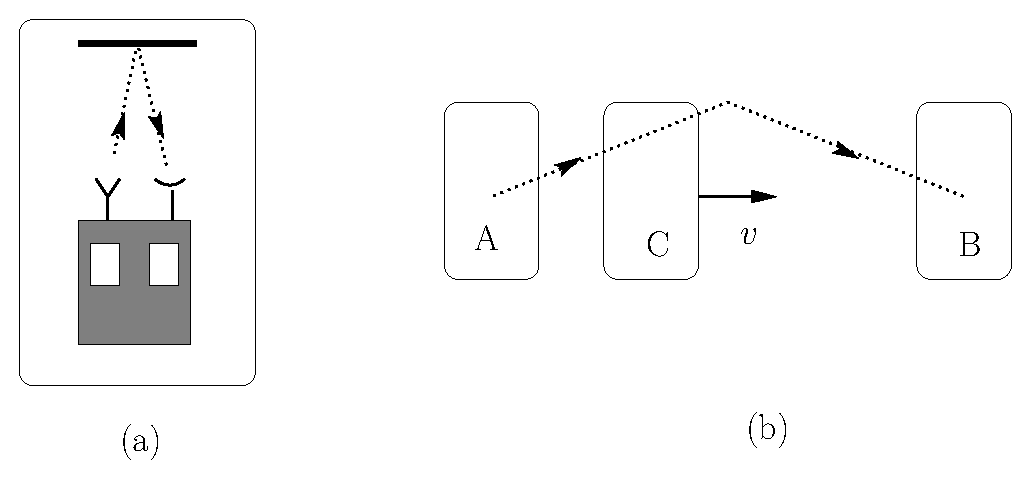
\includegraphics[width=4.5in]{basic_postulates_of_relativity/rel1_clocks.eps}
\end{center}
\caption{(a) A light clock used in the thought experiment described in
  the text. (b) Light clock C passing rest-frame clocks A and B.  The
  dotted line shows the path of C's light pulse as observed in the
  rest frame of A and B.}
\label{fig:light-clocks}
\end{figure}

Suppose clock C emits a light pulse at the exact instant it passes
clock A.  Also suppose that the distance between A and B is such that
clock C passes clock B at the precise instant clock C's reflected
pulse returns to the source.  We therefore have two events: Event \#1
= ``C passes A'' and Event \#2 = ``C passes B.'' We label the time
interval between these two events --- measured by clock C --- as
$\Delta t_C$.  The quantity $\Delta t_C$ is called the {\em proper
  time} interval between the two events; {\bf {\em proper time is
    defined as the time measured on a single clock that is present at
    both events}}.  In the case discussed above, clock C measures the
proper time.  In our particular arrangement, the proper time is
exactly one tick.
   
We now pose the crucial question, the answer to which is the key to
understanding all of special relativity.
\begin{quote}
{\em What is the elapsed time} $\Delta t_{AB}$ {\em as measured by
clocks A and B for clock C to travel from A to B?}
\end{quote}
``Simple,'' you might think.  ``The answer is obviously exactly one
tick, the same as that measured by clock C, right?''  Wrong.  As we
will see, the concepts of absolute time (i.e., everyone and everything
measures the passage of time the say way) is a casualty of the
invariance of the speed of light.
   
For the question posed above to have any meaning, clocks A and B must
be synchronized; i.e., observers in the Earth's reference frame would
say that the two clocks are reading the same time.  (Note: this is not
a trivial matter --- we will discuss synchronization more fully in
Chapter \ref{chapter:relativistic_spacetime}.)  The two-clock time
$\Delta t_{AB}$ is then the difference between the time reading on
clock A at Event \#1 (clock C at clock A) and the time reading on
clock B at Event \#2 (clock C at clock B).
   
In clock C's reference frame, clock A passes C first, and then clock B
passes C.  The time interval between these events is $\Delta t_C$ on
clock C and therefore the light pulse in clock C travels a round-trip
distance equal to $c\Delta t_C$.  But from Fig.~\ref{fig:light-clocks}
this same pulse (the one inside clock C) travels a longer, zig-zag
path when viewed from the frame in which clocks A and B are at rest.
Because of the invariance of the speed of light, {\em this longer
  distance must translate into a longer time interval.}  This means
the round trip time for clock C's pulse is one tick as measured on
clock C, but it is more than one tick when measured on clocks A and B.
In other words, the elapsed time between the event ``C passes A'' and
the event ``C passes B'' is {\em longer} when measured with the two
clocks A and B than when measured with the single clock C.

\begin{figure}[tbp]
  \begin{center}
    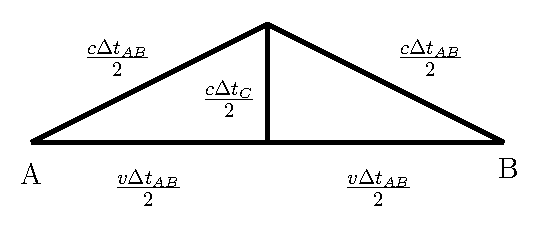
\includegraphics{basic_postulates_of_relativity/rel1_triangle.eps}
  \end{center}
  \caption{Diagram for derivation of the proper time relation.  In 
    this figure $\Delta t_{AB}$ is the elapsed time determined from 
    the clocks A and B, and $\Delta t_C$ is the elapsed time on clock C.}
  \label{fig:rel_triangle}
\end{figure}

How much longer is the time interval $\Delta t_{AB}$ measured on the A
and B clocks than the proper time interval $\Delta t_C$ measured on
clock C?  We can find out by looking at the path taken by the pulse of
light in clock C viewed from C's reference frame and from A and B's
reference frame (see Fig.~\ref{fig:rel_triangle}).  As we've already
seen, in clock C's frame the pulse travels straight up and down along
the vertical line in the figure and the total round-trip distance is
$c\Delta t_C$.  The same pulse, traveling for time $\Delta t_{AB}$
relative to A and B travels the total zigzag distance $c\Delta
t_{AB}$.  Clock C itself travels a distance $v\Delta t_{AB}$ relative
to clocks A and B while the pulse makes one round-trip in C.
Therefore, using the Pythagorean theorem on either small triangle in
Fig.~\ref{fig:rel_triangle}, we find
\begin{equation}
\left(\frac{c\Delta t_{AB}}{2}\right)^2 = 
\left(\frac{c\Delta t_{C}}{2}\right)^2 + 
\left(\frac{v\Delta t_{AB}}{2}\right)^2,
\end{equation}
from which we solve for the proper time $\Delta t_C$ to obtain
\begin{equation}
\Delta t_C = \Delta t_{AB}\sqrt{1 - v^2/c^2}.
\end{equation}
This relation can be written in the general form:

\begin{boxiteq}
{
\begin{equation}
\Delta t_{\rm proper} = \Delta t_{\rm two-clock}\sqrt{1 - v^2/c^2}.
\label{eq:ptr}
\end{equation}
}
\end{boxiteq}

\noindent This very important relation is sometimes called the
``proper time relation'' or the principle of ``time dilation.''
Qualitatively, it expresses the fact that {\bf {\em different
observers measure the passage of time differently depending on their 
relative motion.}}
   
Hidden inside Eq.~(\ref{eq:ptr}) is another result from special
relativity; namely, no object can travel at a speed greater than $c$
relative to any other object or reference frame.  A superluminal speed
($|v| > c$) would result in an imaginary proper time, something that
has no physical meaning.  You will learn later that this speed limit
is imposed by energy considerations as well (it would take an infinite
amount of energy to accelerate an object with mass\footnote{Of course,
a photon of light can be considered an ``object'' that travels at 
a speed $c$, but this is a massless object.  We'll say more about this 
in Chapter \ref{chapter:relativity_pande}.} to a speed $v = c$
relative to an observer, and {\em more} than an infinite amount of
energy to achieve a speed $v > c$).  Therefore, because $|v| \leq c$,
the proper time interval $\Delta t_{\rm proper}$ between two events
is always {\em smaller} than the time $\Delta t_{\rm two-clock}$
measured in a frame that requires two synchronized clocks for
measurement.

   
\begin{example}{Time dilation.}
A father and his daughter are traveling on a train that moves with a 
constant speed of $1.8\times 10^8\units{m/s}$ ($= 0.6c$)
relative to the ground.  They pass a parked VW Beetle at which point
the two of them simultaneously yell, ``Red Punch Buggy!'' and punch each
other on the shoulder.  Three seconds later, the daughter yells,
``Jinx!''  What is the time between these two events according to a
person inside the VW who is waiting for the train to pass?
\solution
The key question ---  who measures the proper time (i.e., the
smaller time interval)?  To answer this, write this down in terms of
events.  Event A $=$ father/daughter punch each other; Event B $=$
daughter jinxes her dad.  In this example, the father/daughter are at
both events (not the person in the car), so they measure the smaller
(proper) time interval, which has already been stated to be $3\units{s}$.  
So, we are given $\Delta t_{\rm proper}$ and we are solving for 
$\Delta t_{\rm two-clock}$, 
which is the time interval measured by the person in the car.
\begin{align}
\Delta t_{\rm proper} &= \Delta t_{\rm two-clock}\sqrt{1-v^2/c^2} \nonumber \\
\Rightarrow \Delta t_{\rm train} &= 
                \Delta t_{\rm VW}\sqrt{1-v^2/c^2}\nonumber \\
\Rightarrow \Delta t_{\rm VW} &= 
                \frac{\Delta t_{\rm train}}{\sqrt{1-v^2/c^2}}\nonumber \\
                   &= \frac{3\units{s}}{\sqrt{1-(0.6c/c)^2}}\nonumber \\
                   &= \frac{3\units{s}}{\sqrt{1-0.6^2}}\nonumber \\
                   &= 3.75\units{s}.
\end{align}
\end{example}

In this example, the father and daughter on the train measured the
proper time because they were at both events, so the time interval is
smaller from their reference frame.  Be careful, though: sometimes the
observer standing on the Earth measures the smaller time interval --- it
all depends on what the events are and who happens to be present at
both of them.
   
Note also that we expressed $v$ as a fraction of the speed of light --- it
makes things a lot simpler to write $v$ in this manner.  We'll say more
about this later

\section{Length contraction}

One thing that will come up repeatedly in this unit is the fact that
relativity breaks down the distinction between distance and time.  In
fact, in relativity, distance and time are really just flip sides of
the same coin.  And as we will see now, you can't change our
conception of time without making a similarly dramatic change in the
way we view distances and length.
   
Consider the following thought experiment: a train is moving on a
track, with Observers A and B at the front and back end of the train.
A and B have measured the length of the train with a long tape measure
that they carry with them on the moving train, and find the length to
be $L_{\rm train}$.  The train goes past Observer C who is standing
next to the track with a stopwatch (see Fig.~\ref{fig:contraction}).
Relative to C in the ``ground reference frame,'' the train is moving
with a speed $v$.  From the train's reference frame, of course, it is
C and the ground that are moving at a speed $v$ in the opposite
direction.
    
   
\begin{figure}[tbp]
\begin{center}
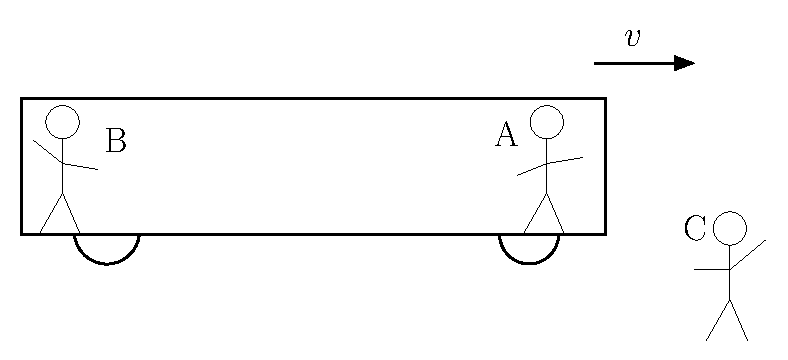
\includegraphics[width=3.5in]{basic_postulates_of_relativity/rel1_train.eps}
\end{center}
\caption{Sketch of train for length contraction thought-experiment.}
\label{fig:contraction}
\end{figure}   
   
Let's say that Observer C wants to measure the length of the train.
He can use his stopwatch to do this: since distance = (speed) $\times$
(time), the length of the train is simply the speed $v$ times the time
interval between when the front of the train passes and when the back
of the train passes.  Let's consider two events: Event A $=$ front of
train passes C; Event B $=$ back of train passes C.  According to
people on the train, the time between the two events $\Delta t_{\rm
  train} = L_{\rm train}/v$, where $L_{\rm train}$ is the
previously-measured length of the train --- this is how far Observer C
moves between the events according to train observers.  But, as we saw
in the previous section, C measures the proper time (since this
observer is at both events), which is a smaller time interval:
\begin{equation}
\Delta t_C = \Delta t_{\rm proper} = \Delta t_{\rm train}\sqrt{1 - v^2/c^2}.
\end{equation}
Based on this result, Observer C now says that the length of the train is 
\begin{align}
 \text{Length} = (\text{speed})\times (\text{time}) &= v\Delta t_C \nonumber \\
                &=  v \Delta t_{\rm train}\sqrt{1-v^2/c^2}  \nonumber \\
                &= L_{\rm train}\sqrt{1-v^2/c^2}.
\end{align}
{\bf {\em The length of the train as measured by an observer by the
side of the track is less than the length of the same train as
measured by people moving with the train.}}

We can write this relation (referred to as the {\bf {\em Lorentz
contraction}} or simply {\bf {\em length contraction}} equation) in
more general terms:

\begin{boxiteq}
{
\begin{equation}    
L_{\rm other} = L_{\rm rest}\sqrt{1-v^2/c^2},
\label{eq:lengthcontract}	
\end{equation}
}
\end{boxiteq}

\noindent where $L_{\rm rest}$ is the length of an object as measured by
observers in a reference frame where that object is at rest, and
$L_{\rm other}$ is the length as measured by observers in a different
reference frame.  Note that an object is always largest when viewed
from its own reference frame, and shrinks when it is viewed as moving.
   
Some comments are in order:  
\begin{itemize}
\item You can't have time dilation without length contraction --- the 
two necessarily go hand-in-hand.  This is a recurring theme of relativity ---
Einstein's theory can't be taken ``a la carte''; rather, it is all or nothing.
Einstein realized that if any single prediction of relativity were
ever refuted, then the entire theory would have to be discarded.  
\item The arguments in this section apply to length components along
the direction of the relative motion.  Components of a length in 
directions perpendicular to the relative motion are not contracted. 
\item Length contraction is not an illusion or merely a matter of
perception.  In the example, the train doesn't just appear to be
smaller from C's reference frame; rather, it  {\em really is
smaller} in that reference frame.  Some of the homework problems and
drill questions will investigate some of the curious properties of
length contraction.
\end{itemize}

\section{Experimental evidence}
   
Most people are skeptical when they first read about the predictions
of special relativity.  This is to be expected, since we do not
experience time dilation or length contraction effects on a daily
basis.  For these effects to be significant, you need relative
velocities that are significant fractions of the speed of light.
Looking at both Eqs.~(\ref{eq:ptr}) and (\ref{eq:lengthcontract}), the
key piece is the stretch factor $\sqrt{1-v^2/c^2}$, which is almost
identically equal to 1.00 for even the fastest velocities that people
ever experience.  This is an important aspect of relativity;
namely, that it obeys classical correspondence, i.e., the results of
relativity agree with Newton's classical results for smaller
velocities.
   
Despite the fact that relativistic effects are almost negligible in
the ``everyday'' phenomena of our personal experience, there is 
copious experimental evidence
that shows that Einstein's predictions are correct.  In every case
where an experiment has tested the theory of relativity, the
experimental results have always agreed precisely with the predictions
of relativity.  Some examples:

\begin{itemize}
\item {\bf Time dilation}.  Time dilation is the most tested aspect of
relativity.  The most direct test was performed by taking two
identical atomic clocks, flying one around the world on a plane and
leaving the other on the ground, then comparing their readings after
the trip.  As predicted by Einstein, the clocks had ticked off
different times, and by precisely the predicted amount.\footnote{Note
that General Relativity plays a role here because the height of a
clock also affects its rate, but the experiments took account of these
general relativistic effects.} Particle decay has also been used to
test time dilation: a type of particle that typically lives for a
certain period of time has been shown to live significantly longer if
accelerated to high speeds (relative to the ground); again, the
difference in times agrees perfectly with relativity.  And the Global
Positioning System (GPS) --- which involves a series of satellites
with precise clocks --- uses relativity extensively to keep the
orbiting clocks synchronized with those in the GPS units on the Earth.
Without relativistic corrections, GPS wouldn't work!
   
\item {\bf The speed of light as a speed limit.}  This result is verified
daily in particle accelerators.  It is fairly straightforward for
scientists to accelerate subatomic particles to speeds close to the
speed of light.  But no matter how much energy is added, the speeds
never make it to or above $c$.  Electrons, in particular, have been
accelerated to speeds $u> 0.99999999999c$, but never up to or above $c$.
   
\item {\bf Length contraction.}  No experimentalist has managed to
accelerate a train to relative speeds large enough to measure length
contraction effects.  (Trust us: you wouldn't want to be anywhere near
a train going this fast.)  But there is experimental evidence for
length contraction: (a) cosmic rays produced at the top of the Earth's
atmosphere somehow manage to make it to the surface of the Earth
before decaying, despite the fact that they are very unstable.  Some
of these particles have lifetimes so short that even traveling at
speeds close to $c$, they would be expected to decay long before they
reach the ground.  This can be explained using length contraction: the
distance from the top of the atmosphere to the Earth's surface is
significantly contracted from their reference frame, so there is no
problem making it to the Earth's surface before
decaying.\footnote{This result can also be explained using time
dilation, of course, because time dilation and length contraction are
really different aspects of the same phenomenon.} (b) Another piece of
experimental evidence comes from electromagnetic theory --- it turns out
that you can explain why an electrical current produces magnetic
effects by applying relativistic length contraction to the stream of
electrons.  The argument is too long to present here (especially since
we haven't covered electricity and magnetism yet), but suffice it to
say that the results agree perfectly with an analysis based on length
contraction.
\end{itemize}
   
There are other experimental tests of other aspects of relativity,
some of which will be discussed later in this unit (when those aspects
are presented).  But, in general, it is worth remembering that
relativity is not a series of different theories, but rather is a
single, coherent, internally consistent theory.  All of the
predictions are inherently related to each other.  So you can't say,
``Well, I'm fine with time dilation but I don't buy length
contraction.''  You simply can't have time dilation without length
contraction --- they are the same thing. So even if there hadn't been
any independent experimental evidence of length contraction (which
there is) there would be very little doubt of its veracity since time
dilation has been verified extensively.

\section{Units and dimensionless velocities}

When working with relativity, it is convenient to express lengths in
terms of distance traveled by light in one unit of time.  A ``light
year'' for instance is the distance that light travels in one year.
An analogy would be to say that the distance between here and New York
City is ``three car hours'' (i.e., it takes 3 hours to get to New York
in a car driving at highway speeds).  In fact, you will often hear
people using time directly to express a distance: ``Oh, it's 3 hours
to New York City from here.''  We will abbreviate these units as lt-s,
lt-min, lt-yr, \dots for light-second, light-minute and light-year,
respectively. Using these units for distance, we can express speeds in
terms of lt-s/s, lt-min/min, lt-yr/yr, etc.  Since the speed of light
$c = 1 \units{lt-s/s} = 1 \units{lt-min/min} = 1 \units{lt-yr/yr} =
\dots$, the speed of a particle in these units is simply the speed
expressed as a fraction of the speed of light.
   
\begin{example}{Units Conversion from lt-s/s to m/s}
  A proton is traveling at a speed of $0.25\units{lt-s/s}$.  Find its speed in
  units of m/s.  \solution Use the fact that $1\units{lt-s/s}$ is equal to
  about $3.00\times 10^8\units{m/s}$.  Then convert units in the
  usual way:
\[ 0.25\units{lt-s/s} \times 
        \frac{3.0\times 10^8\units{m/s}}{1\units{lt-s/s}}
       = 0.75\times 10^8\units{m/s}.  \]
In this example, a particle has a speed $u = 0.25\units{lt-s/s}$.  This same
speed could be expressed as $u = 0.25c$.  In fact, we will typically
express velocities as a fraction of the speed of light $c$.
\end{example}

\newpage

\section*{Problems}
\markright{PROBLEMS}

\begin{problem}
Give a one sentence definition of a meter, using the concept of
a second and the defined value for $c$.  
\end{problem}

\begin{problem}
A proton is traveling at a speed of $4.0 \times 10^7\units{m/s}$.  
How many lt-s/s is this?
\label{prob:rel_units}
\end{problem}

\begin{problem}
A $\pi^-$ meson is traveling at a speed of $0.060\units{lt-s/s}$.  
Convert this speed to m/s. 
\label{prob:rel_units2}
\end{problem}

\begin{problem}
A spaceship moving at constant speed $0.80\units{lt-s/s}$
travels between two planets A and B in $1000\units{s}$, as measured by
synchronized clocks on the planets.  Calculate the elapsed time
according to a clock carried on board the spaceship.  
\end{problem}

\begin{problem}
How fast does a particle have to travel relative to clocks A and
B, which are at rest relative to each other, in order that its elapsed
time as read on a clock moving with the particle is one-tenth the
elapsed time measured on clocks A and B?  Express your answer both in
lt-s/s and in m/s.
\label{prob:time_dilation1}
\end{problem}
  
\begin{problem}
  A meteorite is observed to travel a distance $1.00 \times
  10^5\units{lt-s}$ relative to the Earth in a time of $6.00 \times
  10^5\units{s}$ as measured by Earth observers.  Calculate the
  elapsed time for this trip as measured by a clock carried along on
  the meteorite.
\label{prob:meteorite}
\end{problem}

\begin{problem}
A crew of astronauts travels at a speed of $0.60c$ from Earth to
the nearest star, Proxima Centauri, a distance of $4.0\units{lt-yr}$ 
(as determined by observers on Earth).
   \begin{enumerate}
   \item Calculate how long the trip takes according to observers at
   rest relative to the Earth. 
   \item Calculate the time for the trip as measured by a clock on the
   spaceship. 
   \item Based on your answer to b), calculate the distance from
   Earth to Proxima Centauri as determined by the astronauts using the
   relation ``distance'' $=$ ``speed'' $\times$ ``time'', where 
   distance, speed and
   time are all measured from the astronauts' reference frame.
   \item Calculate the Earth-Proxima Centauri distance from the
   astronauts' reference frame, but this time use length contraction.
   You should end up with the same result as for c).
   \item Think about the results from parts c) and d).  This should
   convince you that length contraction and time dilation are really
   the same thing (i.e., you can't have one without the other).  
   \end{enumerate}
\label{prob:alpha_centauri}
\end{problem}

\begin{problem}
Another spaceship crew wants to make the trip from Earth to
Proxima Centauri in only 2.0 years as measured by clocks on board their
spaceship.  (Recall from the previous problem statement that the 
distance between Earth and Proxima Centauri is $4.0\units{lt-yr}$ 
as determined by observers on Earth.) 
    \begin{enumerate}
    \item How long does the trip take according to Earth-frame observers?
    \item How fast must the astronauts travel relative to Earth? 
    \end{enumerate}
Hint: First, do both parts a) and b) together.  Also, you will need
to express the speed in terms of the unknown travel time according to
Earth-frame observers.  
\label{prob:alpha_centauri2}
\end{problem}

\begin{problem}
You are in a metallic red VW bug stopped at a traffic light.
You see the traffic light turn green, and $2.5\units{$\mu$s}$ later you hear
the car behind you honk its horn.  What is the time between you 
seeing the light change to green and your hearing of the horn honk 
as measured by an 
alien passing by in a ship at a speed $0.9c$?
\end{problem}

\begin{problem}
There is a supergiant star named Betelgeuse\footnote{Betelgeuse
is a supergiant star located in the constellation Orion.  It is very
cool because it could go supernova anytime in the next million years,
and that will be quite a show for us when it does.} which (in the
Earth's reference frame) is $80\units{lt-yr}$ away.  
    \begin{enumerate}
    \item A crew of astronauts is traveling toward Betelgeuse,
    traveling at a speed $0.8c$ relative to the Earth-Betelgeuse
    reference frame.  What is the separation between Earth and
    Betelgeuse in the astronauts' reference frame?
    \item Another crew traveling toward Betelgeuse measures the
    Earth-Betelgeuse distance to be $23\units{lt-yr}$.  How fast is this 
    second crew traveling relative to the Earth?
    \end{enumerate}
\label{prob:betelgeuse}
\end{problem}

\begin{problem}
Betty is standing by the side of a train track when a really
long train approaches traveling at a ridiculously fast speed of $0.9c$.
Thinking quickly, she pulls out her stopwatch, clicks it on when the
front of the train passes and clicks it off when the back of the train
passes.  After standing back up and smoothing down her hair, she notes
that her stopwatch reads $0.0025\units{s}$.  (She has really good reflexes.)
Betty now makes some calculations.
    \begin{enumerate}
    \item According to Betty, how long is the moving train?  (Assume
     that she was warned in advance that the train was going at a
     speed $0.9c$.)
     \item Later that day (not much later), the train reaches its
     destination and stops.  What is the length of the train according
     to people standing next to the (now motionless) train?
     \end{enumerate}
\end{problem}

\begin{problem}
During migration, two fast Arctic terns fly one behind the other
over London at speed $0.8 c$.
%  As they pass the
%border, a guard at the border station notes that
A tourist  sees the birds pass by while looking at the Big Ben clock tower.
She notes that
a time of $12.0\units{ms}$ elapsed on the clock between the first 
bird's passing and the second bird's passing.
    \begin{enumerate}
    \item How much time elapsed between these two events, according to
    the birds?
    \item How far apart are the birds according to the tourists watching the
birds fly by?  
    \end{enumerate}
\label{prob:terns}
\end{problem}

\begin{problem}{\bf Playing Catch on a Train I}\\
{\bf Note:} This is a non-relativistic physics problem.\\
You are riding in a box car of a train that is traveling along the tracks
at $30\units{m/s}$.  You are bored, so you start to play catch with
your friend who is standing on the opposite side of the box car, $5\units{m}$
away from you.  You throw the ball at a speed of $10\units{m/s}$
straight to your friend, who catches the ball; the given speed and direction
are determined in {\em your\/} reference frame.  You may ignore any vertical
motion of the ball.
 \begin{figure}[h]
    \begin{center}
    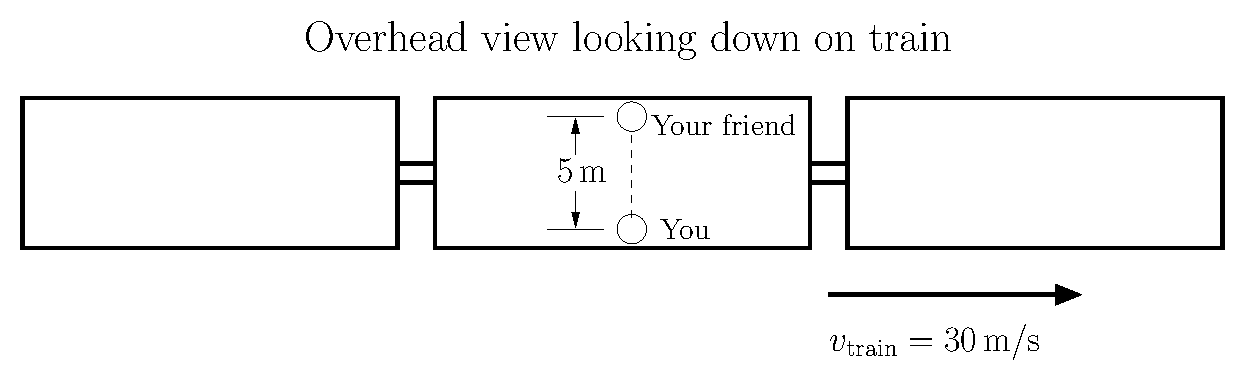
\includegraphics[width=5.5in]{basic_postulates_of_relativity/catch_on_trainI.eps}
    \end{center}
    \caption{Figure for Problem \ref{prob:catch_on_trainI}.  This is
    a top view looking down upon the train.}
    \label{fig:catch_on_trainI}
  \end{figure}
\begin{enumerate}
\item How long does it take for the ball to reach your friend according
to you?
\item How long does it take for the ball to reach your friend according
to an observer standing at rest on the ground?  (This is a dumb question in
classical physics --- if the answer isn't obvious, you're thinking too
hard!)
\item How far does the ball travel according to the observer
standing on the ground?
\item What is the speed of the ball according to the observer
standing on the ground?
\end{enumerate}

\label{prob:catch_on_trainI}
\end{problem}

\begin{problem}{\bf Playing Catch on a Train II}\\
{\bf Note:} This is a non-relativistic physics problem.\\ You are riding in a
box car of a train that is traveling along the tracks at an undetermined
speed.  Once again, you are bored, so you start to play catch with your
friend who is standing on the opposite side of the box car $5\units{m}$
away from you.  (See figure in previous problem.)  You throw the ball
in a horizontal plane at a speed of $10\units{m/s}$ straight to your
friend, who catches the ball.  According to an observer on the ground,
the ball travels a distance of $13.93\units{m}$ between the time you
throw it and the time your friend catches it.  Calculate the speed of
the train along the tracks.
\label{prob:catch_on_trainII}
\end{problem}

\begin{problem}{\bf Photons on a Train}\\
{\bf Note:} This is a relativistic physics problem.\\ Alice is riding
in a box car of a train that is traveling along the tracks at a speed
$v=0.6\units{lt-ns/ns}$.  She just happens to have a light-clock with her
(just like the one illustrated in Fig.~\ref{fig:light-clocks} in Chapter
\ref{chapter:relativityI}).  Alice aligns the clock so that the light
is aimed horizontally directly across the train car, perpendicular to
the motion of the train.  Alice sends a light pulse across the train,
and notices that the light returns to the detector $2\units{ns}$ later.
Alice's friend Bob is standing at rest on the ground as Alice and her
light-clock speed by.  Bob measures the round-trip time for the pulse
of light in Alice's light clock to be $\Delta t_{\rm Bob}$.
\begin{enumerate}
\item What is the speed of the light pulse according to Alice?
\item Determine the distance between the emitter/detector and the mirror
in the light-clock as determined by Alice.
\item  What is the speed of the light pulse according to Bob?  (This is
a dumb question in relativistic physics --- if the answer isn't obvious,
you're thinking too hard!)
\item Determine length of the path traversed by the light pulse according
to Bob {\bf in terms of the unknown time $\Delta t_{\rm Bob}$}.
\item Use the Pythagorean theorem  to find the distance
traveled by the light pulse according to Bob. From this determine
a numerical value for $\Delta t_\text{Bob}$.
% Use your results to determine $\Delta t_{\rm Bob}$.  Do {\bf not}
% use Eq.~(\ref{eq:ptr}) to calculate this result; rather, use the 
% hypotenuse of the right triangle to find the distance the light pulse
% travels according to Bob.

\item Now use Eq.~(\ref{eq:ptr}) to calculate $\Delta t_{\rm Bob}$.
This answer should agree with the answer you determined in the previous
part.
\end{enumerate}
\end{problem}
\newpage
